\section{Probabilidad condicionada}
\subsection{Espacio de probabilidad condicionada}
\begin{itemize}[label=\color{red}\textbullet, leftmargin=*]
	\item \color{lightblue}Objetivo
\end{itemize}
Recalcular la probabilidad de un suceso cuando se dispone de información adicional.

\Ej

Experimento aleatorio = "Lanzamiento dado"

$A=\text{"Obtener un 6"}\longrightarrow P(A)=\dfrac{1}{6}$\\
$B=\text{"Obtener número par"}\longrightarrow P(B)=\dfrac{3}{6}=\dfrac{1}{2}$\\
$P(A/B)=\text{"Probabilidad de obtener un 6 saliendo que salió n$^\circ$ par"}=\dfrac{1}{3}$
\begin{itemize}[label=\color{red}\textbullet, leftmargin=*]
	\item \color{lightblue}Definición
\end{itemize}
Secuencia $(\Omega,\mathcal{S},P)$ espacio de probabilidad. Sea $A\in\mathcal{S}$ y $B\mathcal{S}$ tal que $P(B)>0$. Se define la probabilidad de $A$ condicionada a $B$ como $P(A/B)=\dfrac{P(A\cap B)}{P(B)}$.

\fcolorbox{lightblue}{lightblue!10}{Se define: "Probabilidad de que ocurra $A$ sabiendo que ha ocurrido $B$".}
\begin{itemize}[label=\color{red}\textbullet, leftmargin=*]
	\item \color{lightblue}Proposición
\end{itemize}
Sea $(\Omega,\mathcal{S},P)$ espacio de probabilidad y sea $B$ tal que $P(B)>0$. Entonces, $(\Omega,\mathcal{S},P(\cdot/B))$ es un espacio de probabilidad.\[ \begin{aligned}
	P(\cdot/B):&\mathcal{S}\longrightarrow\R\\
	&A\longrightarrow P(A/B)
\end{aligned} \]
\begin{itemize}[label=\color{red}\textbullet, leftmargin=*]
	\item \color{lightblue}Demostración
\end{itemize}
Ax1,  Ax2 y Ax3 $\longrightarrow$ Se cumplen porque tengo la misma $\sigma$-álgebra $\mathcal{S}$

Ax4 ¿$P(\Omega/B)=1$? $P(\Omega/B)=\dfrac{P(\Omega\cap B)}{P(B)}=\dfrac{P(B)}{P(B)}=1$

Ax5 ¿$P(A/B)\ge0\:\forall A\in\mathcal{S}$? $P(A/B)=\dfrac{P(A\cap B)}{P(B)}\ge0\:\forall A\in\mathcal{S}$

Ax6 ¿$P(A_1\cup A_2\cup \dots/B)=^(A_1/B)+P(A_2/B)+\cdots$? Con $A_i\cap A_j=\varnothing\:\forall i\neq j$.\\
$P(A_1\cup A_2\cup \dots/B)=\dfrac{P\left((A_1\cup A_2\cup \dots)\cap B\right)}{P(B)}=\dfrac{P(A_1\cap B)\cup P(A_2\cap B)\cup \cdots}{P(B)}$\\
$\dfrac{P(A_1\cap B)+p(A_2\cap B)+\cdots}{P(B)}=P(A_1/B)+P(A_2/B)+\cdots$
\subsection{Propiedades}
Además de las propiedades vistas en Tema 3, se cumple las siguientes:
\begin{enumerate}[label=\color{lightblue}\arabic*)]
	\item $P(A/\Omega)=P(A)\longrightarrow P(A/\Omega)=\dfrac{P(A\cap \Omega)}{P(\Omega)}=\dfrac{P(A)}{P(\Omega)}=P(A)$
	\item $P(B/B)=1\longrightarrow P(B/B)=\dfrac{P(B\cap B)}{P(B)}=\dfrac{P(B)}{P(B)}=1$
	\item \lb{Regla del producto:} Si $A$ y $B$ son sucesos tal que $P(A)>0, P(B)>0$ entonces, \[ \begin{rcases}
		P(A\cap B)=P(B)\cdot P(A/B)\\
		P(A\cap B)=P(A)\cdot P(B/A)
	\end{rcases}\longrightarrow\begin{tabular}{l}
	Demostración inmediata usando\\
	definición condicionada
	\end{tabular} \]
\end{enumerate}
\begin{itemize}[label=\color{red}\textbullet, leftmargin=*]
	\item \color{lightblue}Teorema (Probabilidad compuesta)
\end{itemize}
Sea $(\Omega,\mathcal{S},P)$ un espacio de probabilidad y sean $A_1,A_2,\dots,A_n\in\mathcal{S}$ tales que $P(A_1\cap A_2\cap \dots\cap A_{n-1})>0$. Entonces\[ P(A_1\cap A_2\cap \dots\cap A_n)=P(A_1)\cdot P(A_2/A_1)\cdot P(A_3/A_1\cap A_2)\cdot \dots \cdot P(A_n/A_1\cap A_2\cap \dots\cap A_{n-1}) \]Diremos que $\{A_1,A_2,\dots,A_n\}$ es una partición de $\Omega$ si $A_1\cup A_2\cup\dots\cup A_n=\Omega$ y $A_i\cap A_j=\varnothing$.
\begin{itemize}[label=\color{red}\textbullet, leftmargin=*]
	\item \color{lightblue}Demostración
\end{itemize}
Usando la definición de probabilidad condicionada, el término de la derecha quedaría.

\[ \cancel{P(A_1)}\cdot\dfrac{\cancel{P(A_1\cap A_2)}}{\cancel{P(A_1)}}\cdot\dfrac{P(A_1\cap A_2\cap A_3)}{\cancel{P(A_1\cap A_2)}}\cdot~~\cdots~~\cdot\dfrac{P(A_1\cap A_2\cap \dots\cap A_n)}{P(A_1\cap A_2\cap \dots\cap A_{n-1})} \]

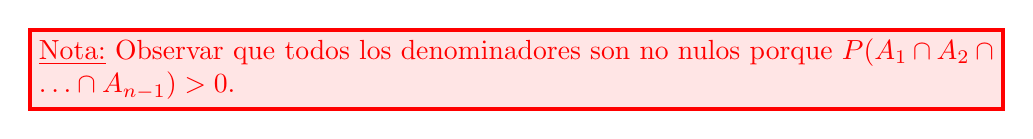
\begin{tikzpicture}
	\node[red, draw=red, fill=red!10, line width=1.5, text width=\textwidth]  {\underline{Nota:} Observar que todos los denominadores son no nulos porque $P(A_1\cap A_2\cap \dots\cap A_{n-1})>0$.};
\end{tikzpicture}

\Ej

Se extraen 3 cartas sin reemplazamiento de la baraja española (40 cartas). Calcular la probabilidad de extraer 3 ases.

$A_i=\text{"Obtengo un As en la $i$-ésima extracción"},\:i=1,2,3$

Me piden $P(A_1\cap A_2\cap A_3)=\lb{\left\{\begin{tabular}{l}
		Teorema de \\
		probabilidad compuesta
\end{tabular}
	\right\}}=\left(\dfrac{4}{40}\right)\cdot\left(\dfrac{3}{39}\right)\cdot\left(\dfrac{2}{38}\right)=\dfrac{1}{2470}$
\begin{itemize}[label=$-$]
	\item Otra forma: \[ \dfrac{\text{casos favorable}}{\text{casos posibles}}=\dfrac{\binom{4}{3}}{\binom{40}{3}}=\dfrac{4}{\frac{40!}{3!37!}}=\dfrac{4}{\frac{40\cdot38\cdot39}{3\cdot 2}}=\dfrac{4\cdot3\cdot2}{40\cdot39\cdot38}=\dfrac{1}{2470} \]
\end{itemize}
\begin{itemize}[label=\color{red}\textbullet, leftmargin=*]
	\item \color{lightblue}Teorema de la Probabilidad Total
\end{itemize}
Sea $(\Omega,\mathcal{S}, P)$ espacio de probabilidad y sean $H_1,H_2,\dots,H_n$ una partición de $\Omega$ con $P(H_i)>0\:\forall i$ y sea $A\in\mathcal{S}$ suceso cualquiera. Entonces: \[ P(A)=P(H_1)\cdot P(A/H_1)+P(H_2)\cdot P(A/H_2)+\cdots +P(H_n)\cdot P(A/H_n). \]
\begin{itemize}[label=\color{red}\textbullet, leftmargin=*]
	\item \color{lightblue}Demostración
\end{itemize}
$A=A\cap\Omega=\lb{\left\{\begin{tabular}{l}
		por ser $(H_1,\dots,H_n)$ partición\\
		de $\Omega$
	\end{tabular}\right\}}=A\cap(H_1\cup H_2\cup \dots \cup H_n)=\lb{\left\{\begin{tabular}{l}
	propiedad\\
	distributiva
	\end{tabular}\right\}}=(A\cap H_1)\cup (A\cap H_2)\cup\dots\cup(A\cap H_n)$

Observar que $(A\cap H_i)$ y $(A\cap H_j)$ son incompatibles o distintos $\forall i\neq j$ por ser $H_i\cap H_j=\varnothing\:\forall i\neq j$.

Tomando probabilidades en la igualdad inicial quedaría \[ P(A)=P(A\cap H_1)+P(A\cap H_2)+\cdots+P(A\cap H_n) \]Regla del Producto $=P(H_1)\cdot P(A/H_1)+P(H_2)\cdot P(A/H_2)+\cdots +P(H_n)\cdot P(A/H_n)$
\begin{itemize}[label=\color{red}\textbullet, leftmargin=*]
	\item \color{lightblue}Teorema (de Bayes)
\end{itemize}
En las condiciones del teorema anterior, se tiene que: \[ \underset{i=1,2,\dots,n}{P(H_i/A)}=\dfrac{P(H_i)\cdot P(A/H_i)}{P(H_1)\cdot P(A/H_1)+P(H_2)\cdot P(A/H_2)+\cdots +P(H_n)\cdot P(A/H_n)} \]
\begin{itemize}[label=\color{red}\textbullet, leftmargin=*]
	\item \color{lightblue}Demostración
\end{itemize}
$ P(H_i/A)=\lb{\left\{\begin{tabular}{l}
		definición probabilidad\\
		condicionada
	\end{tabular}\right\}}=\dfrac{P(A\cap H_i)}{P(A)}=\lb{\left\{\begin{tabular}{l}
	en el numerador aplico la regla del\\
	producto, en el denominador el \\
	Teorema de la Probabilidad Total
	\end{tabular}\right\}}=\dfrac{P(H_i)\cdot P(A/H_i)}{P(H_1)\cdot P(A/H_1)+P(H_2)\cdot P(A/H_2)+\cdots +P(H_n)\cdot P(A/H_n)}$
\begin{itemize}[label=\color{red}\textbullet, leftmargin=*]
	\item \color{lightblue}Nomenclatura
\end{itemize}
$P(H_i)=$ Probabilidad a priori\\
$P(A/H_i)=$ Probabilidad a posteriori

\Ej

Una urna con 3 bolas blancas y 2 negras. Otra urna con 2 bolas blancas y 3 negras. Se lanza un dado y si sale 1 se extrae una bola de la urna 1. En caso, contrario, se extrae de la urna 2.
\begin{enumerate}[label=\color{red}\alph*)]
	\item \lb{Probabilidad de sacar bola blanca.}
	
	$\begin{array}{|c|}
		\begin{array}{l}
			3B\\
			2N
		\end{array}\\ \hline
	\end{array}\qquad\begin{array}{|c|}
	\begin{array}{l}
		2B\\
		3N
	\end{array}\\ \hline
	\end{array}$
	
	$B=$"sacar bola blanca"\\
	$\begin{array}{l}
		U_1=\text{"sacar bola blanca de la urna 1"}\longrightarrow P(U-1)=\dfrac{1}{6}\\
		U_2=\text{"sacar bola blanca de la urna 2"}\longrightarrow P(U_2)=\dfrac{5}{6}
	\end{array}\begin{cases}
	P(B/U_1)=\dfrac{3}{5}\\
	P(B/U_2)=\dfrac{2}{5}
	\end{cases}$
	
	Aplico Teorema de la Probabilidad Total.\\
	$P(B)=P(U_1)\cdot P(B/U_1)+P(U_2)\cdot P(B/U_2)=\dfrac{1}{6}\cdot\dfrac{3}{5}+\dfrac{5}{6}\cdot\dfrac{2}{5}=\dfrac{13}{30}$
	\item \lb{Si sale una bola blanca, probabilidad de que fuera en la urna 1.} \[ P(U_1/B)=\dfrac{P(U_1)\cdot P(B/U_1)}{P(B)}=\dfrac{\frac{1}{6}\cdot\frac{3}{5}}{\frac{13}{30}}=\dfrac{3}{13} \]
	\item \lb{Si sale una bola negra, probabilidad de que fuera en la urna 1.}
	
	$\begin{array}{l}
		P(N)=1-P(B)=1-\dfrac{13}{30}=\dfrac{17}{30}\qquad P(N/U_1)=1-P(B/U_1)=\dfrac{2}{5}\\
		=(U_1/N)=\dfrac{P(U_1)\cdot P(N/U_1)}{P(N)}=\dfrac{\frac{1}{6}\cdot\frac{2}{5}}{\frac{17}{30}}=\dfrac{2}{17}
	\end{array}$
\end{enumerate}
\subsection{Independencia de sucesos}
\begin{itemize}[label=\color{red}\textbullet, leftmargin=*]
	\item \color{lightblue}Definición
\end{itemize}
Sea $(\Omega,\mathcal{S},P)$ un espacio de probabilidad y sean $A,B\in\mathcal{S}$ sucesos. Diremos que $A$ y $B$ son \lb{independientes} si $P(A\cap B)=P(A)\cdot P(B)$

$\bboxed{P(A/B)=\dfrac{P(A\cap B)}{P(B)}\longrightarrow P(A\cap B)=P(B)\cdot P(A/B)=P(A)\cdot P(B/A)}$
\begin{itemize}[label=\color{red}\textbullet, leftmargin=*]
	\item \color{lightblue}Propiedad
\end{itemize}
\begin{enumerate}[label=\color{lightblue}\arabic*)]
	\item $A$ y $B$ son independientes.
	\item $P(A/B)=P(A)$
	\item $P(B/A)=P(B)$
\end{enumerate}
\begin{itemize}[label=\color{red}\textbullet, leftmargin=*]
	\item \color{lightblue}Demostración trivial usando regla de productos:
\end{itemize}
\begin{enumerate}[label=\color{lightblue}\arabic*)]
	\item Si $A$ y $B$ son independientes
	\begin{enumerate}[label=\color{lightblue}1.\arabic*)]
		\item $A$ y $B^c$ son independientes
		\item $A^c$ y $B$ son independientes
		\item $A^c$ y $B^c$ son independientes
	\end{enumerate}
\end{enumerate}
\begin{itemize}[label=\color{red}\textbullet, leftmargin=*]
	\item \color{lightblue}Definición
\end{itemize}
\begin{wrapfigure}[2]{r}{0.5\textwidth}
	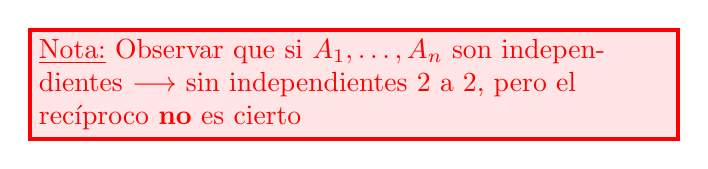
\begin{tikzpicture}
		\node[red, draw=red, fill=red!10, line width=1.5, text width=8cm] {\underline{Nota:} Observar que si $A_1,\dots,A_n$ son independientes $\longrightarrow$ sin independientes 2 a 2, pero el recíproco \textbf{no} es cierto};
	\end{tikzpicture}
\end{wrapfigure}

Diremos que $A_1,\dots,A_n$ son \lb{independientes} si se cumple que: 

$P(\underset{i\in I}{\cap}A)=\underset{i\in I}{\pi}\cdot P(A_i)\quad \forall I\le \{1,2,\dots,n\}$
\begin{itemize}[label=\color{red}\textbullet, leftmargin=*]
	\item \color{lightblue}Teorema (de Bayes generalizado)
\end{itemize}
Sea $(\Omega,\mathcal{S}, P)$ un espacio de probabilidad y sea $\{H_1,\dots, H_n\}$ partición $\Omega$. Sean $A$ y $B\in\mathcal{S}$ con $P(A\cap H_i)>0\:\forall i=1,\dots,n$ \[ P(B/A)=\dfrac{\displaystyle\sum_{i=1}^{n}P(H_i)\cdot P(A/H_i)\cdot P(B/A\cap H_i)}{\displaystyle\sum_{i=1}^{n}P(H_i)\cdot P(A/H_i)} \]
\begin{itemize}[label=\color{red}\textbullet, leftmargin=*]
	\item \color{lightblue}Demostración
\end{itemize}
\begin{center}
	$P(B/A)=\dfrac{P(B\cap A)}{P(A)}$\qquad\begin{minipage}[l]{6cm}
	\lb{Aplico el teorema de la Probabilidad Total tanto a numerado como denominador}
\end{minipage}
\end{center}


